\subsection{Approaches to fairness in SQF}

Before going into detail about a specific study, we provide a tabular overview of the different approaches to fairness in the SQF data. We will go into more depth into two of them in the following.

\begin{table}[h]
    \centering
        \begin{tabular}{|m{2cm}|m{3cm}|m{2.5cm}|m{3.5cm}|m{2.8cm}|}
            \hline
            \textbf{Authors} & \textbf{Task} & \textbf{Model} & \textbf{Fairness Metric} & \textbf{Results} \\
            \hline
            \cite{kallus2018} 
            & Predict prob. of innocence (no weapon) 
            & Log. Regression 
            & Equal Opportunity, Equalized Odds 
            & Bias against PoC \\ 
            \hline
            \cite{rambachan2016} 
            & Possession of contraband
            & Log. Regression 
            & No explicit fairness metric; evaluate prediction function properties 
            & No bias against PoC\\
            \hline
            \cite{Badr2022DTFANSP} 
            & Predict probability of arrest 
            & Log. Regression, RF, XGBoost, GNB, SVC 
            & Balanced Accuracy, Stat. Parity, Equal Opportunity, Disparate Impact, Theil Index 
            & No bias against PoC \\ 
            \hline
            \cite{Khademi2019FADMELC} 
            & Predict probability of arrest 
            & Weighted regression models
            & FACE causal fairness (group), FACT fairness (individual) 
            & No group bias, but individual bias \\ 
            \hline
            \cite{goel2016} 
            & Predict possession of weapon 
            & (Penalized) Log. Regression 
            & No explicit fairness metric; group-wise hit rates 
            & Bias against Black and Hispanic\\ 
            \hline
        \end{tabular}
        \caption{Overview of SQF-related fairness studies. This table summarizes findings from five key studies evaluating the fairness of the stop-and-frisk policy. Depending on the task and model used, the studies reach different conclusions.}
        \label{tab:sqf_summary}
\end{table}

% \subsection{Sources of bias in the SQF data}
One of the main challenges with the NYPD's data is that, when evaluating the fairness of stop-and-frisk as a policing strategy, various tasks can be formulated to address the question. Only some of them are suitable to make conclusions about the fairness of the stop-and-frisk policy as a whole.\par
Like \cite{Badr2022DTFANSP}, we trained a classifier to predict arrests and used group metrics to assess fairness. However, given that we also trained a "fair" classifier on data from 2011, but the stop-and-frisk practice was officially declared unconstitutional for 2004 to 2012, the task we (and \cite{Badr2022DTFANSP}) chose, is not a reliable indicator of the overall fairness of the policy.\par
To answer the question of fairness in stop-and-frisk other studies take a step back and identify a problem with how the data is generated. They formalize and acknowledge that the discrimination in SQF does not solely lie in the outcome of the stop but the decision to stop someone in the first place.


\subsection{Residual unfairness}

In their paper \textbf{Residual Unfairness in Fair Machine Learning from Prejudice Data} \cite{kallus2018} conceptualize the problem as shown in \autoref{fig:selection_bias}.
A person is defined by their sensitive feature $(A)$ and non-sensitive features $(X)$. For each person in the population of interest a police officer decides whether to stop them $(Z = 1)$ or not $(Z = 0)$. This mechanism can be seen as a category of selection bias and, referring back to the feedback loop (\autoref{fig:biasLoop}), is introduced by the user.\par
In the SQF context, we can imagine that the police are generally more suspicious towards PoC than white people, resulting in more stops of the former. Alternatively, one could argue that they are more likely to stop individuals in high-crime areas, which happen to be mostly low-income neighbourhoods largely populated by PoC.\par
Naturally, we can only know the outcome $Y \in \{0, 1\}$ of a stop for the individuals who were stopped. This can create a situation in which the training data produced by the biased decision policy is not be representative for the population the algorithm will be deployed on.
\cite{kallus2018} distinguish between target population and training population in such scenarios. The target population is the one on which we want to use the ADM on while the training population are the observations the biased decision policy chose to include in the sample and on which the algorithm is trained.\par
The problem for fairness in this case is that fairness adjustments of the learner (trained on the biased sample) do not translate to its deployment on the target population. Even fairness-adjusted classifiers can discriminate against the same group that has historically faced discrimination (\cite{kallus2018}). They call the remaining disparities in fairness metrics after fairness adjustments have been made \textbf{residual unfairness}.\par
% The indicator $T \in \{0, 1\}$ tell us whether a person belongs to the target population. If $T = 1$ constantly, it means that the algorithm should be deployed for the entire population of NYC.\\
At this point, we refer back to \autoref{fig:race_distributions}. The left plot shows a clear difference between the racial distribution in the SQF data and the city as a whole. In terms of race, the sample is clearly not representative for NYC\footnote{It can be questioned whether it makes sense to require the SQF sample to be representative for the population of NYC. It might make more sense to require that it is representative of the population of \textit{criminals} in NYC.}. At the same time the estimated borough-specific crime rates also differ from the distribution of stops per borough as seen in the right plot.\par
\cite{kallus2018} demonstrate that their theoretical findings are reflected in the SQF data. Their task is to predict a person's innocence. They define innocence as not carrying an illegal weapon and guilt as carrying one. The reasoning behind this approach is that the discriminated group is the one more frequently falsely accused of possessing an illegal weapon. The authors find that non-white individuals are indeed more often wrongfully classified as guilty. Even after applying a post-processing strategy to achieve equalized odds, unfairness against PoC persists when the classifier is used on NYC’s overall target population.
\newpage
\begin{figure}[htpb]
    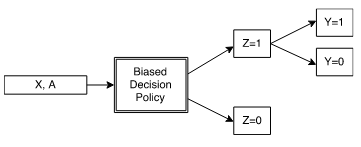
\includegraphics[width=0.5\textwidth]{../figures/selection_bias.png}
    \caption{Selection bias in the SQF data, as conceptualized by \cite{kallus2018}. The true label is only known for the stopped individuals $(Z = 1)$.}
    \label{fig:selection_bias}
\end{figure}

\subsection{Bias in, bias out?}

Another perspective is offered by \cite{rambachan2016} in their paper \textbf{Bias In, Bias Out? Evaluating the Folk Wisdom}.
While the main message of \cite{kallus2018} is that even fairness adjusted classifiers exhibit the "bias in, bias out" mechanism \cite{rambachan2016} argue that it depends on the chosen classification task.

Similar to \cite{kallus2018} they are interested in whether a person carries a contraband $Y \in \{0, 1\}$. The paper assumes the police is a taste-based classifier against African-Americans. This means they hold some form of prejudice against the group of African-Americans that influences their decision to stop a member of this group. More precisely, they see the biased-decision policy in the decision to \textit{search} someone.\par
When we previously defined the biased selection mechanism as $Z=1$ corresponding to stop and $Z=0$ corresponding to no stop, this study sees the biased decision policy in the decision to search someone, which then should be denoted as $Z^*=1$ for search and $Z^*=0$ for no search. Though the studies select different variables for the biased decision policy their conceptual frameworks remain comparable.
Again, only on searched people a contraband can be found. The goal is to estimate the possession of a contraband $Y$, but we estimate this from $Y | Z^*=1$.\par

In contrast to \cite{kallus2018}, the authors of this paper argue that the classifier shows the opposite effect; instead of continuing to discriminate the previously disadvantaged group, the classifier exhibits \textit{less} bias as the prejudice against African-Americans increases.\par
As the police becomes more biased towards African-Americans, they search them more leniently. This means that many innocent African-Americans are included in the searched observations. Consequently, the model learns on average lower risk scores for African-Americans. Essentially, the data for African-Americans becomes more noisy, which lowers the predicted probabilities for this group. The authors call this mechanism \textbf{bias reversal}.

\cite{rambachan2016} continue to examine alternative classification tasks that could be constructed from the SQF data. In their second scenario, they train an algorithm to predict whether to search someone in the first place ($Z^* \in \{0, 1\}$). Now the search becomes the target and in this case \textbf{bias inheritance} is observed, meaning the classifier continues to discriminate the historically disadvantaged group.\par
The same happens for a two stage classification task that first predicts whether to search someone and if they searched someone if the individual carries a contraband ($Y \cdot Z^* \in \{0, 1\}$). What happens here is that as more of the stopped African Americans are also searched, the algorithm learns to associate search with more with African Americans than with white people and thus in the future also predicts higher probabilities for a search for African Americans. This is the \textbf{bias inheritance} mechanism.
We can see parallels to this paper to our own case study in the sense that, PoC indeed have lower risk scores (\autoref{fig:fairness_density}, left) and are relatively speaking less often predicted as arrested as white individuals.

As seen in \autoref{tab:sqf_summary} there are more studies that have worked with the SQF data, each with a unique approach to the question of fairness. \cite{Khademi2019FADMELC} are also interested in whether the decision to arrest an individual, after a stop has been made, is discriminatory with respect to race. They design two causal fairness methods, namely the Fair on Average Causal Effect (FACE) and the Fair on Average Causal Effect on the Treated (FACT), to estimate the causal impact of race on the outcome. Their notions of fairness are based on counterfactual reasoning, utilizing Inverse Probability Weighting and Matching to estimate the quantities of interest.
While one of their metrics finds that the odds of being arrested after a stop are higher for Black-Hispanics than for white individuals, the other metric does not show any racial discrimination.\par
\cite{goel2016}, on the other hand, focus on the prediction of the possession of a weapon. They construct a statistical model to account for location specific crime rates and developments of criminal activity over time. After controlling for these factors, the authors conclude that Black and Hispanic individuals are disproportionately often involved in low-risk stops.
